\documentclass[a4paper,12pt]{article}


\usepackage{amssymb,amsmath,array}
\usepackage{hyperref}
\usepackage{bm}
\usepackage{graphicx}

\usepackage[a4paper, left=3cm, right=2.5cm, top=3cm, bottom=3cm]{geometry}
% language and encoding
\usepackage[utf8]{inputenc}
\usepackage[T1]{fontenc}
\usepackage[english]{babel}
% this package load language specific quotes and enables you to write
% \enquote{text} instead of "`text"' or something like that.
\usepackage{csquotes}
\newcommand{\ts}{\textsuperscript}

% Write initials inside the right margin
\newcommand{\initials}[1]{\marginpar{\quad\texttt{#1}}}

\title{Report of the 3\ts{rd} project}
\author{First group member (FGM), Second group member (SGM), \and
Third group member (TGM)}

% could removed
\date{Submission by 31\ts{st} January 2021}


\begin{document}

\pagenumbering{gobble}

\pagestyle{myheadings}
\markright{First group member, Second group member, Third group member}
    
\maketitle

\begin{center}
    \textbf{Tutorial: Monday 12-14, Tutor: tutor's name}
\end{center}

\section{Introduction}
This is a template for a report. You may use the outline or change it freely. There are no directives.

\section{Data Set}
\initials{TGM}

\section{Foundations}

\subsection{Methods}
Which models are used? How do they classify/differ? 

\subsection{Evaluation}
Which evaluation methods are used?

\subsection{Feature Selection}
\initials{FGM}

\section{Experiments}

\subsection{Set-Up}
How are the experiments designed? What choices did you make, why?

\subsection{Results}
Overview of the results.
\initials{SGM}


\begin{figure}[h]
\centering
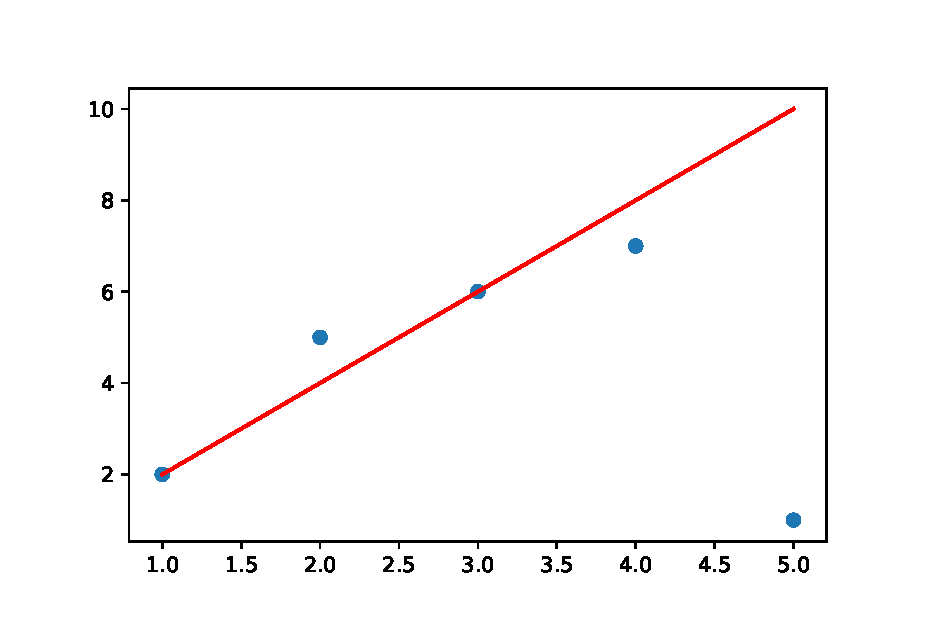
\includegraphics[width=0.8\textwidth]{plot}
% where an .eps filename suffix will be assumed under latex, 
% and a .pdf suffix will be assumed for pdflatex; or what has been declared
% via \DeclareGraphicsExtensions.
% E.g. you can use plt.savefig('./plot.eps') in your python script
\caption{Data and regression line from sheet 5. For saving the figure we use the command \texttt{plt.savefig('./plot.eps')}.}
\label{fig_res}
\end{figure}


You can refer to Figure~\ref{fig_res}.
\begin{table}[h]
\caption{An example of a table}
\label{tab_example}
\centering
% Some packages, such as MDW tools, offer better commands for making tables
% than the plain LaTeX2e tabular which is used here.
\begin{tabular}{c||c|c|c}
Data & Method 1 & Method 2 & Method 3\\
\hline\hline
data 1 &0.54 & 0.6& 0.98\\
\hline
data 2 &0.74 & 0.54& 0.48\\
\hline
data 3 &0.82 & 0.71& 0.67
\end{tabular}
\end{table}
You can also refer to Table~\ref{tab_example}. Do not wonder that the floats are somewhere else in the document.
\initials{FGM}

\subsection{Analysis}
Why do your results make sense in the context of the work? Did you find something surprising?

\section{Discussion}
Short summery and future work.
\initials{SGM/TGM}

\end{document}